%----------------------------------------------------------------------------
\chapter{Tervezési kritériumok meghatározása}
\label{sec:LatexTools}
%----------------------------------------------------------------------------

A diploma dolgozatomban, ahogy a bevezetőben is említettem egy telemanipulátor geometriai, elektronikai és szoftveres tervezését, ezeknek az elemek elkészítésest és működését fogom bemutatni. Az első lépés a felsorolt feladatok teljesítéséhez, hogy egy átfogó szempont rendszert hozzak létre. Ez abban segített nekem, hogy a tervezési lépéseknél figyelembe véve az eredmény így egységes és a meghatározott funkciókkal volt ellátva.  

\section{Telemanipulátorokról általánosan}
%----------------------------------------------------------------------------

Tartalmi tisztázásképpen szeretném előbb bemutatni, hogy általános megfogalmazásban mi a telemanipulátor. Ez egy, olyan eszközöket magába foglaló robotikai rendszer, amely lehetővé teszi egy operátor\footnote{Egy személy, aki a mozgás utasítások kiadását közvetlenül végzi} számára, hogy közvetve irányítson és mozgásutasításokat adjon egy robotkarnak vagy manipulátornak. Az ilyen típusú rendszerek jellemzően két jól elhatárolható részből állnak, egy vezérlőpanelből (továbbiakban HMI - Human Machine Interface) és egy fizikai manipulátorból, amellyel a mozgás utasítás cél pozícióját vagy orientációját lehet megadni a robotkar vagy manipulátoroknak.

A telemanipulátoros rendszerek célja, hogy a valós robot mozgatás és a operátor pozíciója helyben ne legyen korlátozva. Lehetővé tegye azt, hogy a robotkar vagy manipulátor közvetlen vezérlését biztonságosabb, nyugodtabb vagy az én általam elkészített telemanipulátor esetében szempont ok alapján egy szoftveres réteg mögül tegye meg. A telemnaipulátorok főalkalmazási területe, ahol szükséges az hogy az operátor és a robotkar térben független lehessen egymástól, ezért ezek az eszközök széles körben alkalmazhatók különböző iparágakban és területeken. Például az űrkutatásban és az űrtörmelék, vagy minta gyűjtésben használják. Az orvostudományban telemanipulátorok segítségével végezhetnek távoli műtéteket és beavatkozásokat. Az ipari területen például gyártásban használják ezeket a megoldásokat nehezen programozható pályák megvalósítására vagy nagy fokú precizitást igénylő munkafolyamatok elvégzésére.

Az alkalmazási területtől függően mennyire terjedelmes, de általános egy telemanipulátor rendszernek számos elvárásnak kell megfelelnie, hogy biztonságosan tudjuk alkalmazni. A geometriától indulva ergonomikusak kell lennie, mivel közvetlenül az operátor keze által vannak a mozgatási parancsok kiadva és ha önmagában a telemanipulátor kezelése gondot okoz, akkor a mozgatás se lesz kielégítő. A szoftveres rendszernek a sebessége a másik kritérium, hogy a rendszernek adott mozgás utasítás és a tényleges mozgás között minimális legyen az eltérés. Ez két általánosan megfogalmazott elvárás önmagában a tervezési lépésekre is meglehet fogalmazni ilyeneket.

A telemanipulátor rendszerek különböző szenzorokat (erő, távolság vagy szögérzékelés) vagy mozgás detektáló rendszereket (képfeldolgozás) használnak, hogy pontos és alapos vezérlést biztosítsanak az operátor számára. Az előrehaladó technológiák, például a virtuális valóság és a vezetéknélküli rendszerek, további lehetőségeket kínálnak a telemanipuláció területén.

Összességében a telemanipulátor rendszerek lehetővé teszik az ember és a robot együttműködését, és hozzájárulnak a térben korlátok nélkül "távoli" helyeken történő feladatok hatékony és biztonságos elvégzéséhez. Ezáltal a telemanipuláció előnyös lehet olyan helyzetekben, ahol emberi jelenlét nem kívánatos vagy nem lehetséges, de mégis szükség van az emberi kézügyességre és irányításra.

\section{Szakdolgozatban elkészített telemanipulátor}
%----------------------------------------------------------------------------

A tervezési elvárások meghatározásának alapja a alapszintű képzésem Szakdolgozatában dokumentált hat szabadságfokú telemanipulátor. Az eszköz tervezése volt az első önálló mérnöki munkám, amelynek eredményeképpen sikerült egy átfogó projektet bemutatnom. Ez telemanipulátor egy egyszerű egytagú karokból és csuklókból összeállított eszköz. Az eszköz elkészítésének koncepciója az volt, hogy a hatodik csuklóra helyezhető legyen egy tetszőleges geometria, amelynek a Tool Counter Point (rövidítve TCP)\footnote{Tool counter point, ami egy definiált pontja a endeffektornak egy viszonyítási koordináta rendszerben.}-jának térben való elmozdulását mérni tudjam a karok egymáshoz viszonyított csuklószögeinek mérésével. Az alábbi képen az elkészült eszköz látható (\ref{fig:Szakdoga_csipeszes}).

\begin{figure}[!ht]
\centering
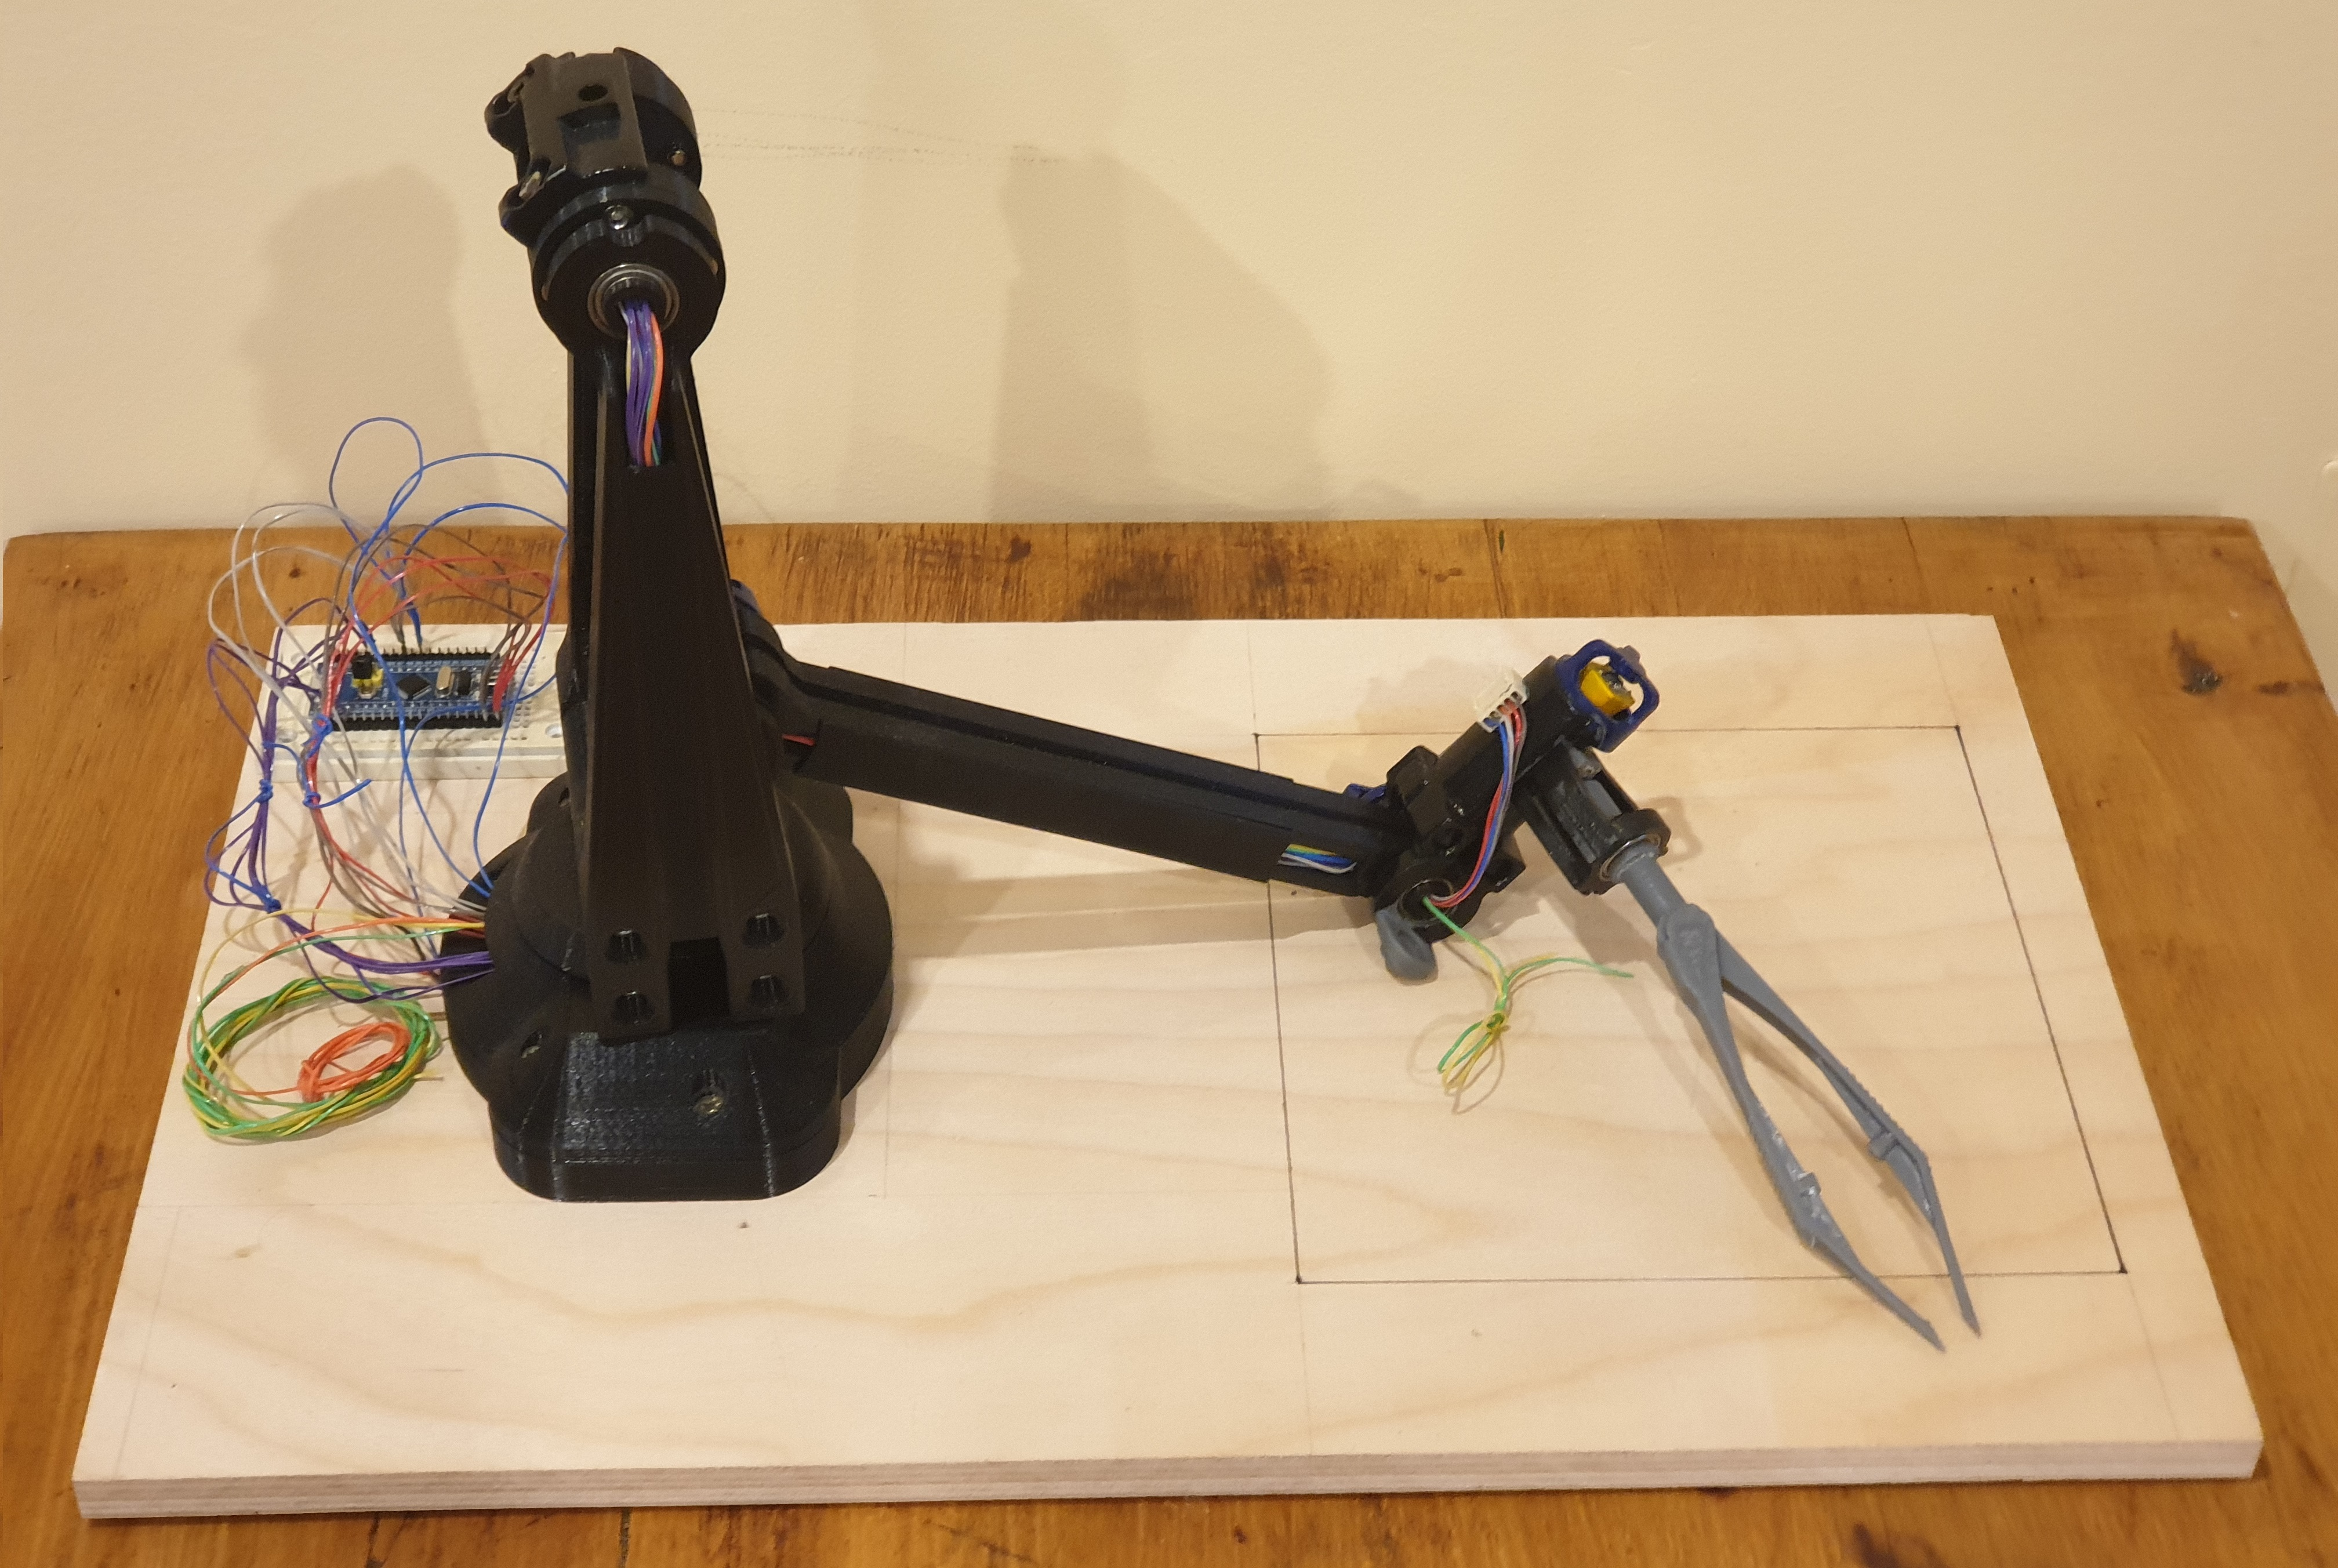
\includegraphics[width=110mm, keepaspectratio]{figures/Szakdoga/0_v_4_csipeszes}
\caption{Szakdolgozatomban elkészített telemanipuláto}
\label{fig:Szakdoga_csipeszes}
\end{figure}

A telemanipulátor 3D nyomtatással lett elkészítve. Ez a prototípus készítési módszer egy manapság már a mérnöki munka alapjának tekinthető főleg a olcsóbb 3D nyomtató eszközök elterjedésével. Az általam használt nyomtatási technológia az alkatrészek nyomtatására ebben az esetben FDM\footnote{Fused Deposition Modeling - A nyomtatási technológia a hőre lágyuló polimerekkel képes 3D-s objektumokat nyomtatni. Az FDM nyomtatók azzal az alapelvvel működnek, hogy szobahőmérsékleten szilárd hőre lágyuló polimert 180$^{\circ}$- 300$^{\circ}$C-ra melegítve ömledéket állapotba kerülnek és a kívánt helyre lehet juttatni lineáris vezetékrendszer segítségével.}, viszont néhány alkatrész, mint például a szenzortartó elkészítéséhez SLA\footnote{StereoLithography Apparatus - modellteret UV aktív gyantával tölti fel. A nyomtatási térben egy síklapra építi fel a tárgyat úgyhogy, az belemerül egy gyantával teli kádba, ahol a megfelelő rétegvastagságú folyékony gyanta réteget UV lézerrel térhálósítja és köti adhézióval az előző réteghez} módon működő nyomtatót használtam. 

A telemanipulátor karok csatlakozásánál mindenhol csapágyakat használtam, ezzel biztosítva az egy tengelyűséget és az ellenállás mentes elfordulást. A vezetékezésben igyekeztem mindenhol tengelyen átlépő vezetékezést tervezni, amit nem akadályozza a rendszer mozgatását.

A mikrovezérlővel begyűjtött szögértékek továbbítottam egy szimulációs rendszernek, amiben igyekeztem megfelelő számításokkal egy virtuális robotkart mozgatni. Végeredményben az adatokkal végzett számításokat nem sikerült maradéktalanul elvégezni. A szakdolgozat megírásának pillanatában nem voltam kellően felkészülve kinematikai számítások terén és egy hibás egyenlet rendszert írtam fel, aminek az eredménye ként a kiszámított koordináták amiket a robotnak követnie kellett volna hibásak voltak. Ezt később Mester képzésen projekt feladatom kapcsán korrigáltam.

\begin{figure}[!ht]
\centering
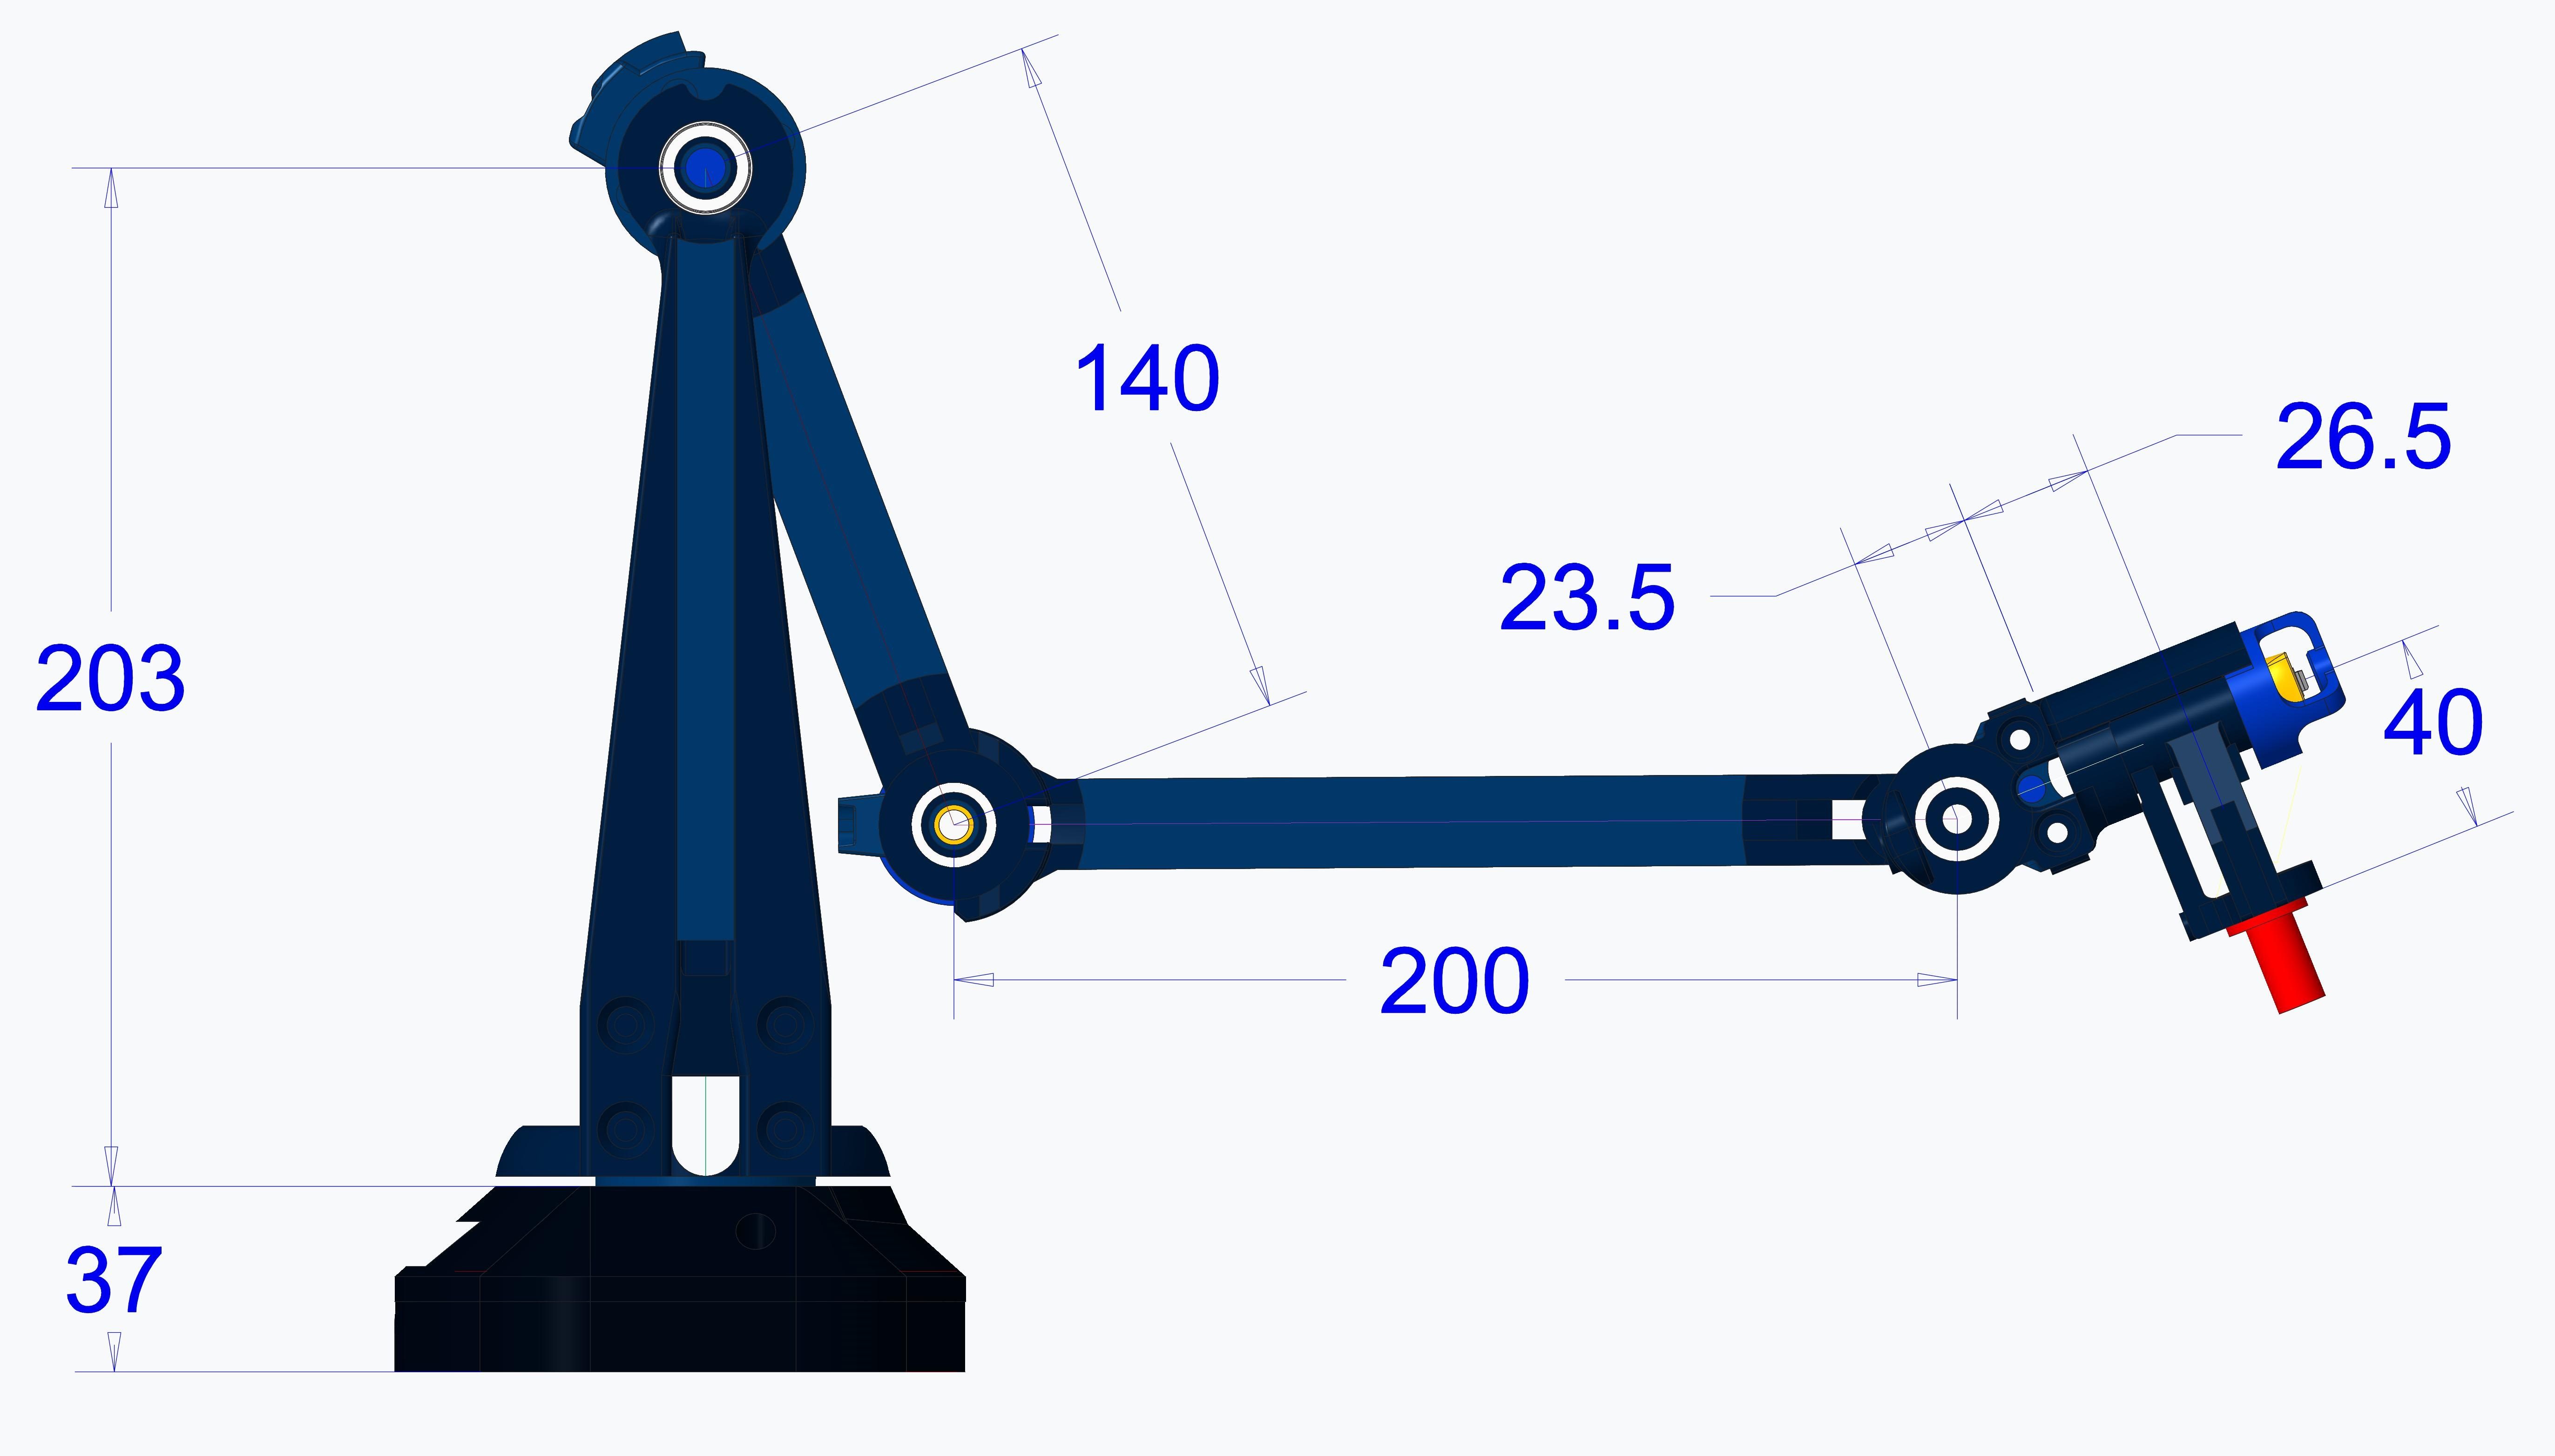
\includegraphics[width=110mm, keepaspectratio]{figures/Szakdoga/00_v_4_kar}
\caption{Szakdolgozatomban elkészített méreteinek bemutatása}
\label{fig:Szakdoga_csipeszes}
\end{figure}

Végeredményben a szakdolgozatomban elkészített telemanipulátor az akkor meghatározott elvárásoknak tökéletesen megfelelt, viszont sok helyen koncepcionális és egy igen komoly számítási hibát tartalmazott. Mester képzésemen az itt felmerülő hibákat céloztam meg első körben kijavítani és az ehhez szükséges elvárásokat a következő fejezetben bemutatom.

\section{Újratervezési szempontok}
%----------------------------------------------------------------------------

A szakdolgozatomban a újra tervezési szempontokat csoportosítás nélkül fogalmaztam meg, ami kissé általánosított megfogalmazást eredményezett, amelyek a következőek voltak:

\begin{enumerate}
\item A manipulátor minél többféle eszköznek a rögzítését és mozgatását tegye lehetővé.
\item Az eszközök a munkatere: $200[mm]x200[mm]x200[mm]$
\item A end-effektorra illesztett szerszámok használatát ne nehezítse a manipulátor súlya.
\item Az eszköz geometriáját úgy kell kialakítani, hogy 3D nyomtatási technológiákkal legyártható legyen
\item A csuklóknál csapágyazást kell alkalmazni.
\item Az eszköz kábelezését minél inkább el kell rejteni.
\end{enumerate}

A diploma dolgozatom esetében is fontosnak éreztem ilyen, pontokat megfogalmazni, de ezt csoportosítva teszem meg a következő alfejezetek alapján. A szakdolgozatban megtervezett és részletesen bemutatott telemanipulátor számomra legnagyobb hibája, hogy túl helytakarékos. Méret és tömeget általában utolsóként szokás racionalizálni. Nincs elég hely az esetleges új funkcióknak és ha esetleg az egyik szenzor meghibásodik vagy másikat kell felhelyezni szinte a teljes eszköz újra kell kábelezni. Programozási tekintettben már említett hiba mellett a mikrovezérlő memóriájában extra tárhely nincs, így itt se lehetséges új funkciók implementálása. Így sokkal célzottabban lehetséges vizsgálni már a különböző problémákat a későbbiekben. Ezt követően illetve egy funkcionális módosítást mutatok be, mielőtt a következő fejezetben a már új telemanipulátor tervezési lépéseit tárgyalnám.

\subsection{Geometriai újratervezési szempontok}

A geometria újratervezése előző telemanipulátor karjainak méretei a kényelmes használat ellenére is túl rövidnek érződtek. A munkatér széle közelében már majdnem végállásban tudtak lenni a karok. Ezért ezeket mindenképpen nagyobbakra kell tervezni.

A kábel csatorna volt a legnagyobb gond. Ezt ugyan egy alapos számítással a kábelek szám, vastagsága alapján választottam meg, de pont emiatt új kábel behúzása nehezen vagy egyáltalán nem kivitelezhető. Az új karok esetében semmilyen formában nem szerettem volna kompromisszumot vállalni ezen a fronton, úgyhogy a megtervezett kar kereszt metszetének több mint $80\%$-át kábel csatornává kell alakítani.

Az ellensúlyos gravitációs hatásából származó terhelés kompenzációjának - amiről a következő fejezetben részletesen kitérek - újragondolása. A szakdolgozatom esetében az összes csukló esetében ezt szerettem volna megvalósítani, de koránt sem a leghatékonyabb.

\subsection{Jelfeldolgozó rendszer újratervezési szempontok}

A jelfeldolgozó rendszer újra tervezése nem volt szükség. A szakdolgozatban bírálatában megfogalmazott bypass kondenzátor használatának lehetőségét viszont megvizsgáltam, így új szenzorokat készítettem kiegészítve ezzel a komponenssel. A mikrovezérlőnél viszont a perifériáinak száma és a memória mérete kevésnek bizonyult. Így ezen a területen egy más, nagyobb kapacitású mikrovezérlő kiválasztását tűztem ki célul.

\subsection{Szoftveres újratervezési szempontok}

A jelfeldolgozó rendszertől kapott csuklószögeket felhasználó programmal szemben a legfontosabb elvárás, hogy hosszú távon valósidejű lefutást támogatnia kell. Ez azért fontos, mert a KUKA robot kollaboratív robotjainak vezérléséhez ez élőkövetelmény.

A korábban említett számítási hiba kijavítása egyértelmű cél volt a szakdolgozatomat alapul véve, de ezt nem követlenül a diplomamunkám keretein belül végeztem el.

\subsection{Sebészeti eszközök vezérlése}
%----------------------------------------------------------------------------

Röviden szeretnék kicsit kitérni arra, hogy a szakdolgozatomban látható ténylegesen modellezett sebészeti eszközöket a diploma dolgozatom esetében nem készítettem el. A cél ugyan az, hogy egy olyan rendszert hozzak létre, ami sebészeti eszközök mozgatását tegye lehetővé robotkarok végén, viszont a rendszer elkészítéséhez nem szükséges már a tesztelésénél ezt használni. A szakdolgozatban látható telemanipulátor végén a csipesz és a szike modell megnehezítette a koordináták ellenőrzését és azt detektálni, hogy mi következik szöghibákból és mi a egyedi end-effektor nem tökéletes ergonómiájából ered. Az se elhanyagolható, hogy a dolgozatban a sebészeti eszköz tökéletesítése önmagában kitudná tölteni egy teljes diploma munkát.

A diploma dolgozatom címében megfogalmazott sebészeti eszközök figyelembe vannak véve a következőkben bemutatásra kerülő telemanipulátor tervezése közben. A szakdolgozatomtól eltérően nem konkrétan a telemanipulátor end-effektorára vonatkozik, hanem a robotkar hatodik csuklójára helyezett eszközre, amit majd a későbbiekben könnyedén lehet ezzel az eszközzel vezérelni.